\documentclass[../report.tex]{subfiles}
\begin{document}
\section{Scheduled Attendance Taking Services}
The attendance taking functionality will be implemented as Android background services that are scheduled to run at the time the session will start. Four different services will be implemented for each of the following functions: opening attendance, closing attendance, advertising attendance tokens, and scanning for devices advertising attendance tokens. The first two services will only run on a device with lecturer credentials. On app startup, the services will be scheduled by an Android AlarmManager.

\section{Custom GATT Profile}
\label{sec:gatt-profile}
A custom GATT profile (dubbed Beam Profile) will be utilised for data transfer between two devices using the app. The Beam Profile contains one custom GATT service (Beam Service) which contains one characteristic, known as Attendance Token, that holds a string value generated as the hash of a lecture session ID. The value of this characteristic can be read by the GATT client, written by the GATT server, and the GATT client can be notified of changes in the characteristic.
\begin{figure}[H]
\centering
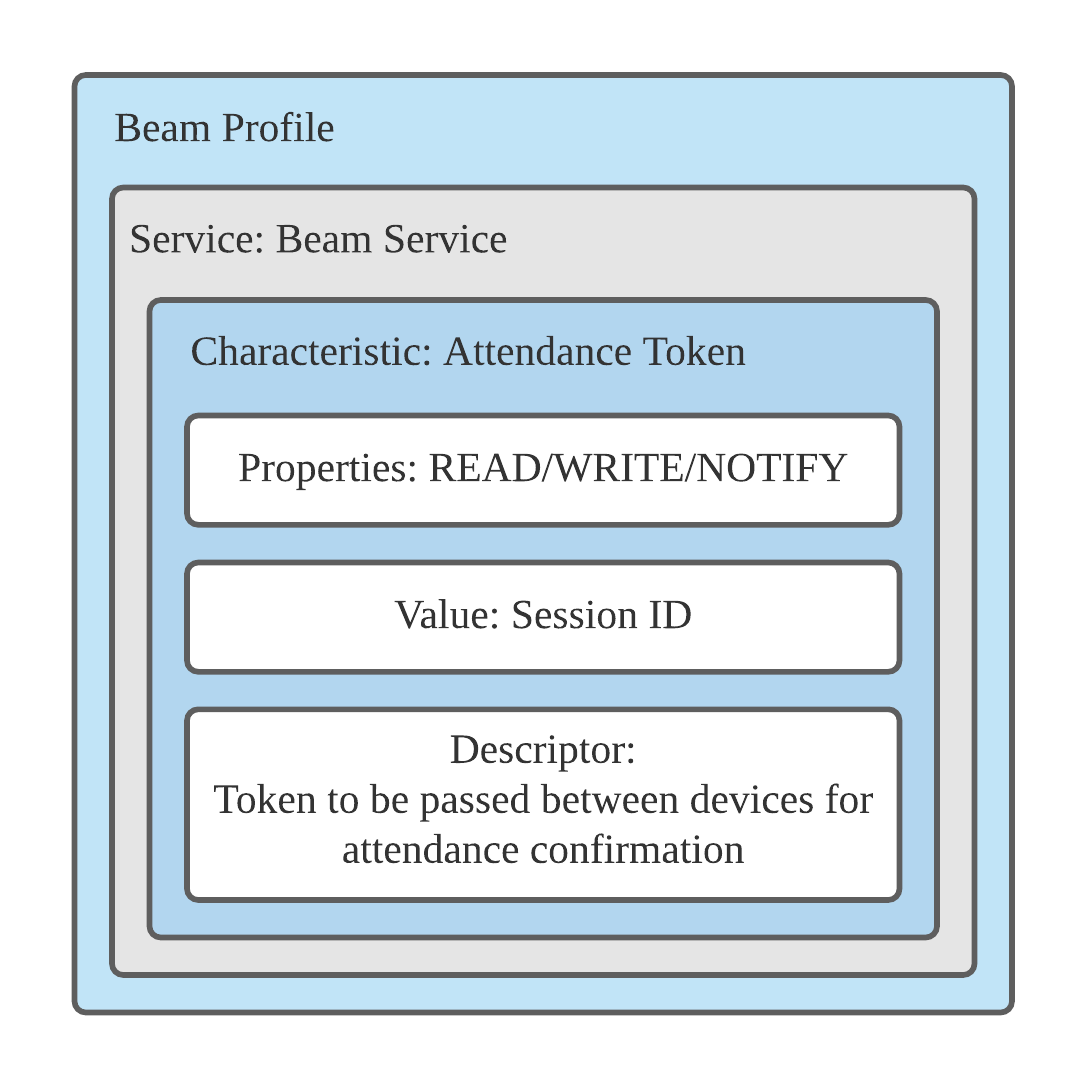
\includegraphics[width=.5\textwidth]{./images/05-02-beam-profile.png}
\caption{Custom GATT Profile}
\label{fig:beam-profile}
\end{figure}

Regarding the peripheral role in the app, the lecturer’s device acts as the first peripheral device. The session ID will be written into the service characteristic. The device will then advertise the Beam Service UUID and wait for connection request from a central device. Once a connection is established, the peripheral acts as the GATT server. Whenever the central device (GATT client) requests to read the value of the characteristic, the server will send a response containing the value. This is how the attendance token is passed between devices.

Regarding the central role in the app, the students’ devices are central devices by default. Once the session has started (based on OS time), the central device will begin scanning for devices that advertise the Beam Service UUID. Once it detects one, it’ll initiate a connection and begin acting as the GATT client. The device will immediately request to read the value of the characteristic within the service. Upon receiving the attendance token, the value is compared to that in the database. Once attendance has been taken, the device closes the connection and switches to a peripheral role.

\section{Database and Web Hosting Choice}
The database used by the app will be Firebase Realtime Database, which is a cloud hosted database whereby data is stored as a JSON tree. All clients share one Realtime Database instance. The data stored by the app is estimated to take up a few GBs of space and only basic querying is required by the app. Additionally, only one instance of the database is needed for all clients. Thus, Firebase recommended Realtime Database as a better choice compared to Firebase Cloud Firestore, a NoSQL relational database, which is better suited for apps that require multiple databases, advanced querying, and hundreds of GBs to TBs of space. Firebase was chosen over other web services (such as Amazon Web Services) because it’s hosting services are free (to a certain degree) and the API is estimated to be easier to learn and work with.

The website is hosted using Firebase Hosting: \url{https://beam-5845a.web.app/}. Email for authentication is admin@nottingham.edu.my and the password is \textit{password}.

\section{Firebase Authentication Design}
There are three types of user accounts: student, lecturer, and admin. Student and lecturer accounts grant permission to access the application, while admin accounts grant access to the administration website. Each student and lecturer accounts will have their own User ID stored in Firebase Authentication. The User ID will be used to query the database to search to student or lecturer details. The admin accounts are created on the console by the team and cannot be created in other way.

\section{User Interface Navigation}
\subsection{Website}
\begin{figure}[H]
\centering
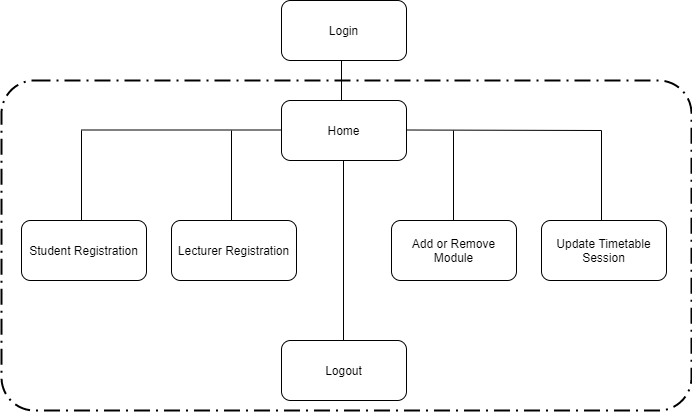
\includegraphics[width=\textwidth]{./images/05-05-web-nav.png}
\caption{Sitemap of administration website. Components  inside the dotted box belong to a single-page application}
\label{fig:beam-profile}
\end{figure}

\subsection{Application}

\section{Use Case Diagrams}
\subsection{Website}
\begin{figure}[H]
\centering
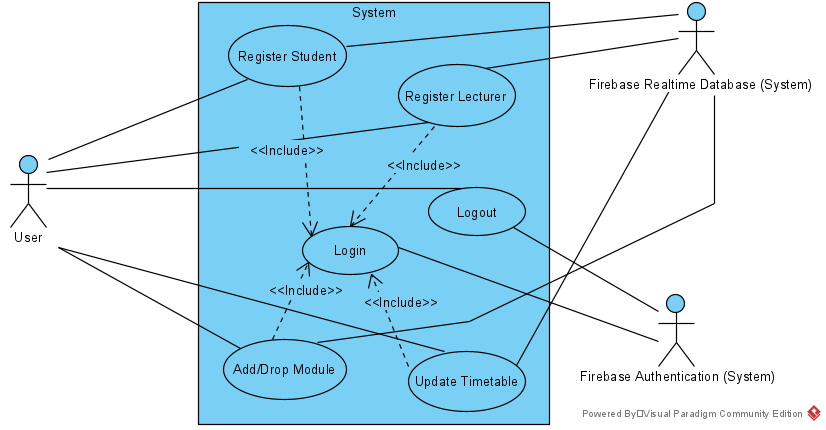
\includegraphics[width=\textwidth]{./images/05-06-web-use-case.png}
%\caption{Use case diagram of website}
\label{fig:web-use-case}
\end{figure}

\subsection{Application}
\textbf{TODO}

\section{Sequence Diagrams}
\subsection{Website}
\subsubsection{Login}
\begin{figure}[H]
\centering
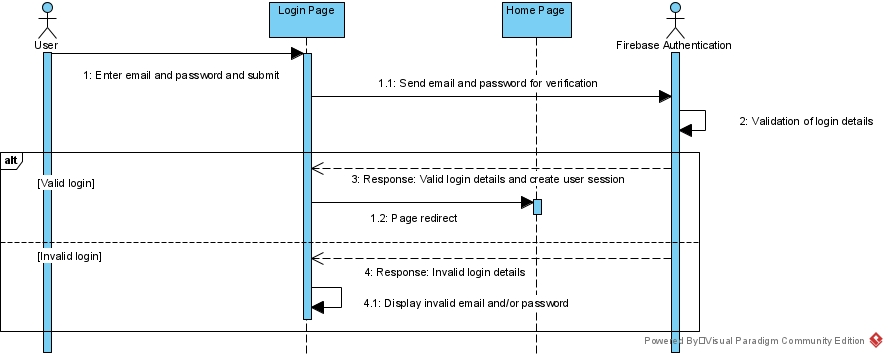
\includegraphics[width=\textwidth]{./images/05-07-web-login.png}
\label{fig:web-login-seq}
\end{figure}

\subsubsection{Student Registration}
\begin{figure}[H]
\centering
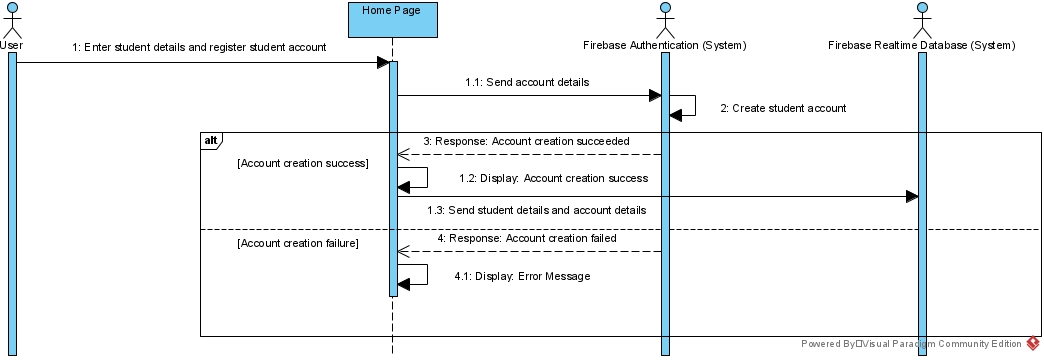
\includegraphics[width=\textwidth]{./images/05-07-web-student-reg.png}
\label{fig:web-student-seq}
\end{figure}

\subsubsection{Lecturer Registration}
\begin{figure}[H]
\centering
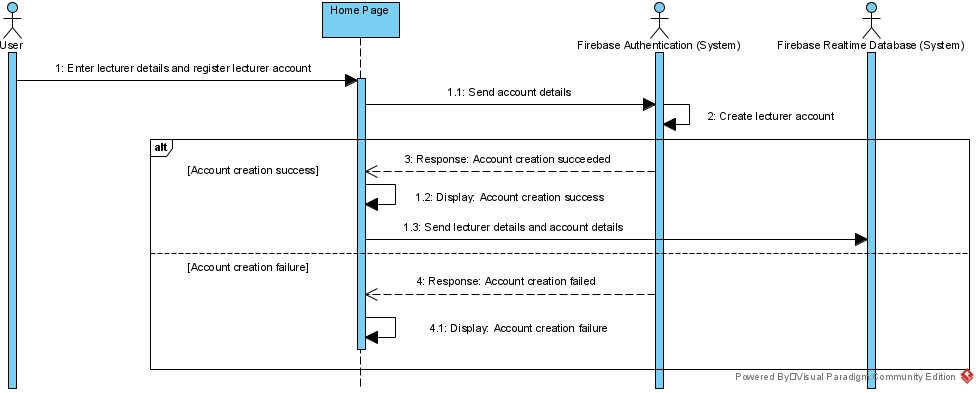
\includegraphics[width=\textwidth]{./images/05-07-web-lec-reg.png}
\label{fig:web-lec-seq}
\end{figure}

\subsubsection{Update Module Information}
\begin{figure}[H]
\centering
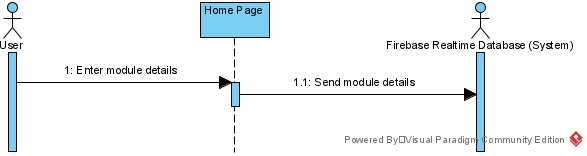
\includegraphics[width=\textwidth]{./images/05-07-web-module.png}
\label{fig:web-module-seq}
\end{figure}

\subsubsection{Update Timetable}
\begin{figure}[H]
\centering
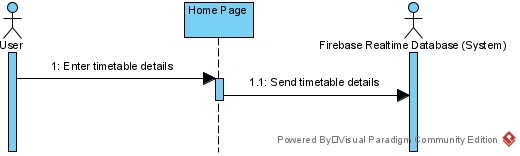
\includegraphics[width=\textwidth]{./images/05-07-web-timetable.png}
\label{fig:web-timetable-seq}
\end{figure}

\subsubsection{Logout}
\begin{figure}[H]
\centering
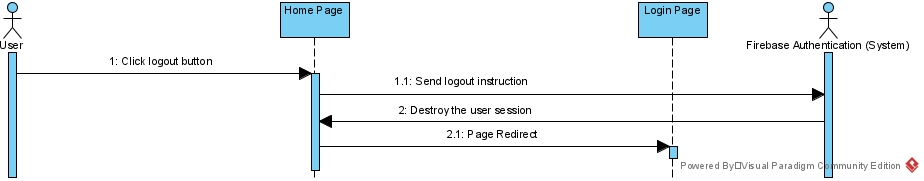
\includegraphics[width=\textwidth]{./images/05-07-web-logout.png}
\label{fig:web-logout-seq}
\end{figure}

\subsection{Application}

\subsubsection{Application Start}
\begin{figure}[H]
\centering
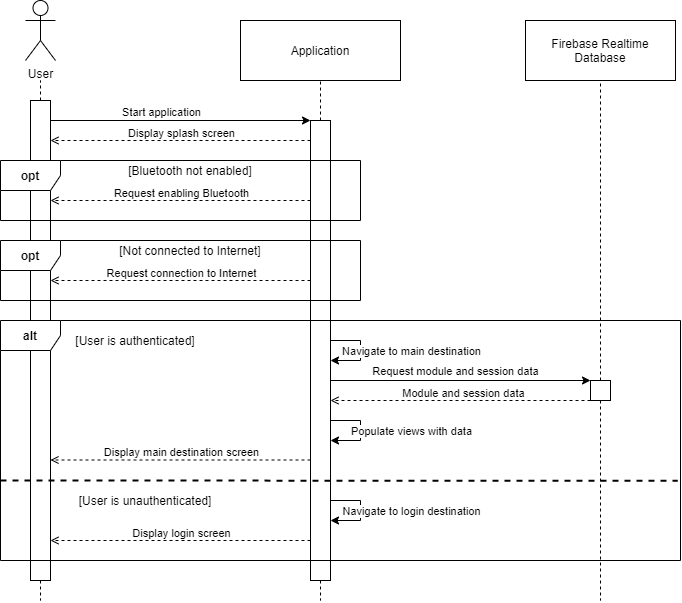
\includegraphics[width=\textwidth]{./images/05-07-app-start.png}
\label{fig:app-start-seq}
\end{figure}

\subsubsection{Login}
\begin{figure}[H]
\centering
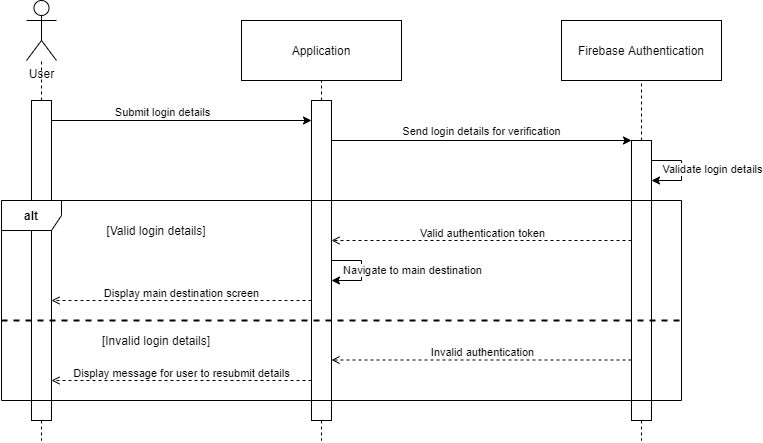
\includegraphics[width=\textwidth]{./images/05-07-app-login.png}
\label{fig:app-login-seq}
\end{figure}

\subsubsection{Attendance Taking}
\begin{figure}[H]
\centering
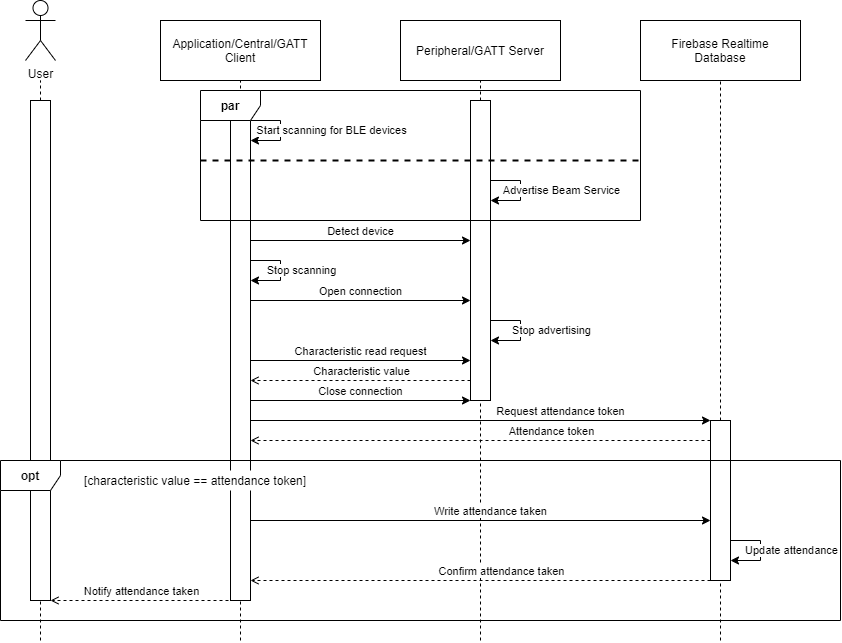
\includegraphics[width=\textwidth]{./images/05-07-app-attendance.png}
\label{fig:app-attendance-seq}
\end{figure}

\section{Firebase Realtime Database Design}
\begin{figure}[H]
\centering
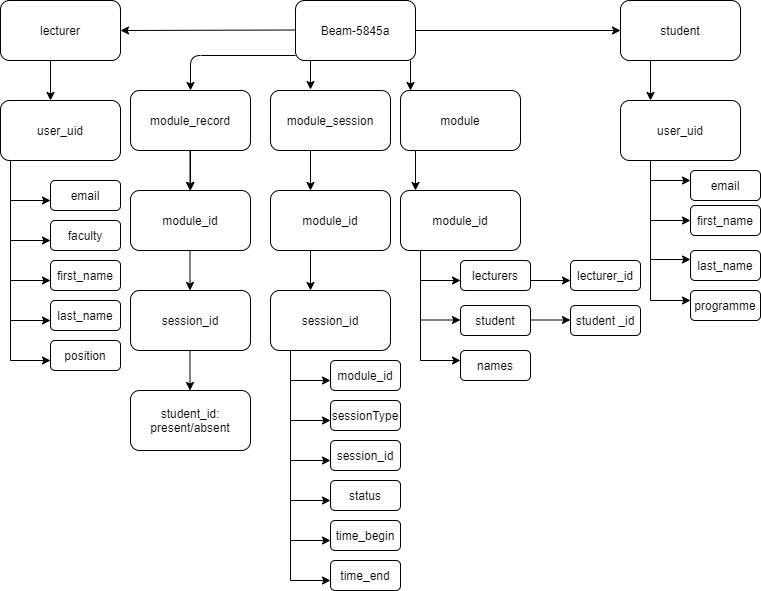
\includegraphics[width=\textwidth]{./images/05-08-database-1.png}
\caption{Database design part 1}
\label{fig:database-design-1}
\end{figure}

The \textit{lecturer} node groups the lecturer details by \textit{user\_uid}, which will be fetched to populate the profile in the app. The \textit{module\_record} node stores the students who attended an academic session by \textit{module\_id}. The app will calculate the percentage of students who attended the session. The \textit{module\_session} node groups each session by their module. The \textit{module} node groups module details by \textit{module\_id}. The \textit{student} node groups the student details by \textit{user\_uid}, which will be fetched to populate the profile in the app.

\begin{figure}[H]
\centering
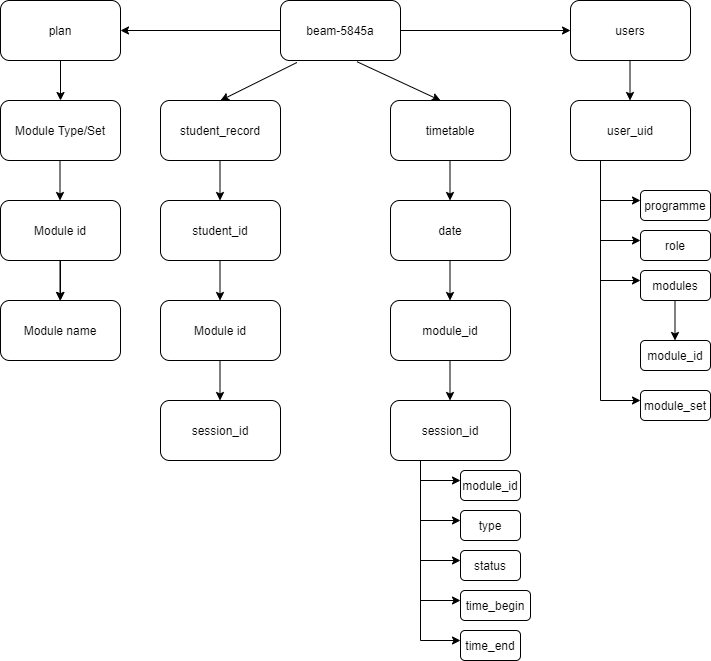
\includegraphics[width=\textwidth]{./images/05-08-database-2.png}
\caption{Database design part 2}
\label{fig:database-design-2}
\end{figure}

The \textit{plan} node stores the modules by programme. Modules in a programme are group by module type or set. Module type such as Core and Elective are applicable for students, while module set groups the modules taught by a lecturer. Grouping modules in this way allows the admin to perform only one data entry (by type or set) instead of entering each module one-by-one. The \textit{student\_record} node stores all attended academic sessions of a student, grouped by module id. The \textit{timetable} node stores each academic session and its module id for every date when there is an academic session. The \textit{user} node stores important identification details. The \textit{programme} node groups all the modules a student is taking in an academic plan. The \textit{role} node identifies whether a user is a student or lecturer. The \textit{module} set groups all the modules a lecturer is teaching. 
\end{document}


